\newpage
\section{Project Plan}
% \subsection{Product Perspective}
\subsection{Objectives}
The primary objective of this project is to successfully design, develop, and deploy the Converge scheduling system. By the end of the development lifecycle, the project aims to achieve the following measurable goals:
\begin{enumerate}
    \item \textbf{Automate the Booking Workflow:} To drastically reduce the estimated 1 to 2 hours of daily administrative overhead  by replacing manual spreadsheet filtering and repetitive messaging with an automated matching engine.
    \item \textbf{Eliminate Scheduling Conflicts:} To implement a commute-aware algorithm and automated room allocation system that mathematically guarantees zero double-bookings and enforces realistic cross-branch travel buffers for instructors.
    \item \textbf{Enhance Operational Visibility:} To deliver a centralized, interactive web dashboard that provides business owners and administrators with a single, real-time source of truth for branch operations.
    \item \textbf{Implement a Scalable Architecture:} To engineer a robust backend utilizing a Modular Monolith and Hexagonal Architecture, ensuring the core scheduling domain is testable, highly maintainable, and prepared for future organizational scaling.
\end{enumerate}

\subsection{Type of System Users and the Users’ Characteristics}
\mytable{|X[0.2,c]|X[l]}{
{User Type} & Description \\

Admin &
the operators who manage course registrations and schedule bookings based on the incoming requests from parents.
\\

Parent &
the users who provide the subject that they want their child to learn to the admin.

} \\
\textbf{User Journey}
\begin{itemize}
    \item \textbf{As is:} A parent contacts the admin to book a class. The admin has to manually search through a cluttered Excel spreadsheet to find an open time slot. If the time works, the admin then has to manually calculate the teacher's travel time between branches and act as a middleman, sending multiple LINE messages back and forth to confirm with everyone. Even after all this manual work, they might arrive at the branch only to find no physical room is actually available.
    \item \textbf{To be:} A parent contacts the admin to book a class. The admin simply inputs the request into Converge. The system instantly auto-matches the available teacher and student , automatically adds the travel time for the teacher , and permanently locks in a physical room. The booking is confirmed accurately in seconds, completely cutting out the messy spreadsheets and group chats.
\end{itemize}

\subsection{Acronyms and Definitions}
\mytable{|X[0.2,c]|X[l]}{
Acronyms & Description \\

Admin &
The operators who manage course registrations and schedule bookings based on the incoming requests from parents.
\\

API &
\textbf{Application Programming Interface}\cite{api_ref}; used in the context of REST API for communication between the frontend and backend.
\\

Commute Buffer &
An automatically calculated travel time inserted between an instructor's consecutive classes at different physical branches.
\\

DDD &
\textbf{Domain-Driven Design}\cite{ddd_ref}; a software design approach focused on modeling the system based on the core business domain.
\\

Hexagonal Architecture &
A backend architectural pattern that keeps the core scheduling domain portable and testable in isolation from the web framework and database.
\\

Modular Monolith &
A deployment architecture where the system is deployed as a single unit but internally structured into well-defined modules.
\\

Parent &
The users who provide the subject that they want their child to learn to the admin.
\\

REST &
Representational State Transfer\cite{rest_ref}; the architectural style used for designing the system's web API.
\\

SaaS &
\textbf{Software as a Service}\cite{saas_ref}; a software distribution model mentioned as out-of-scope for this project.
\\

SDLC &
Software Development Life Cycle; the framework used for planning, creating, testing, and deploying the software.
\\

XP &
Extreme Programming; an Agile software development methodology focused on software quality, combined with Kanban for this project.
\\
}

\newpage
\subsection{System Architecture}
\textbf{1.Hexagonal Architecture}
\begin{center}
    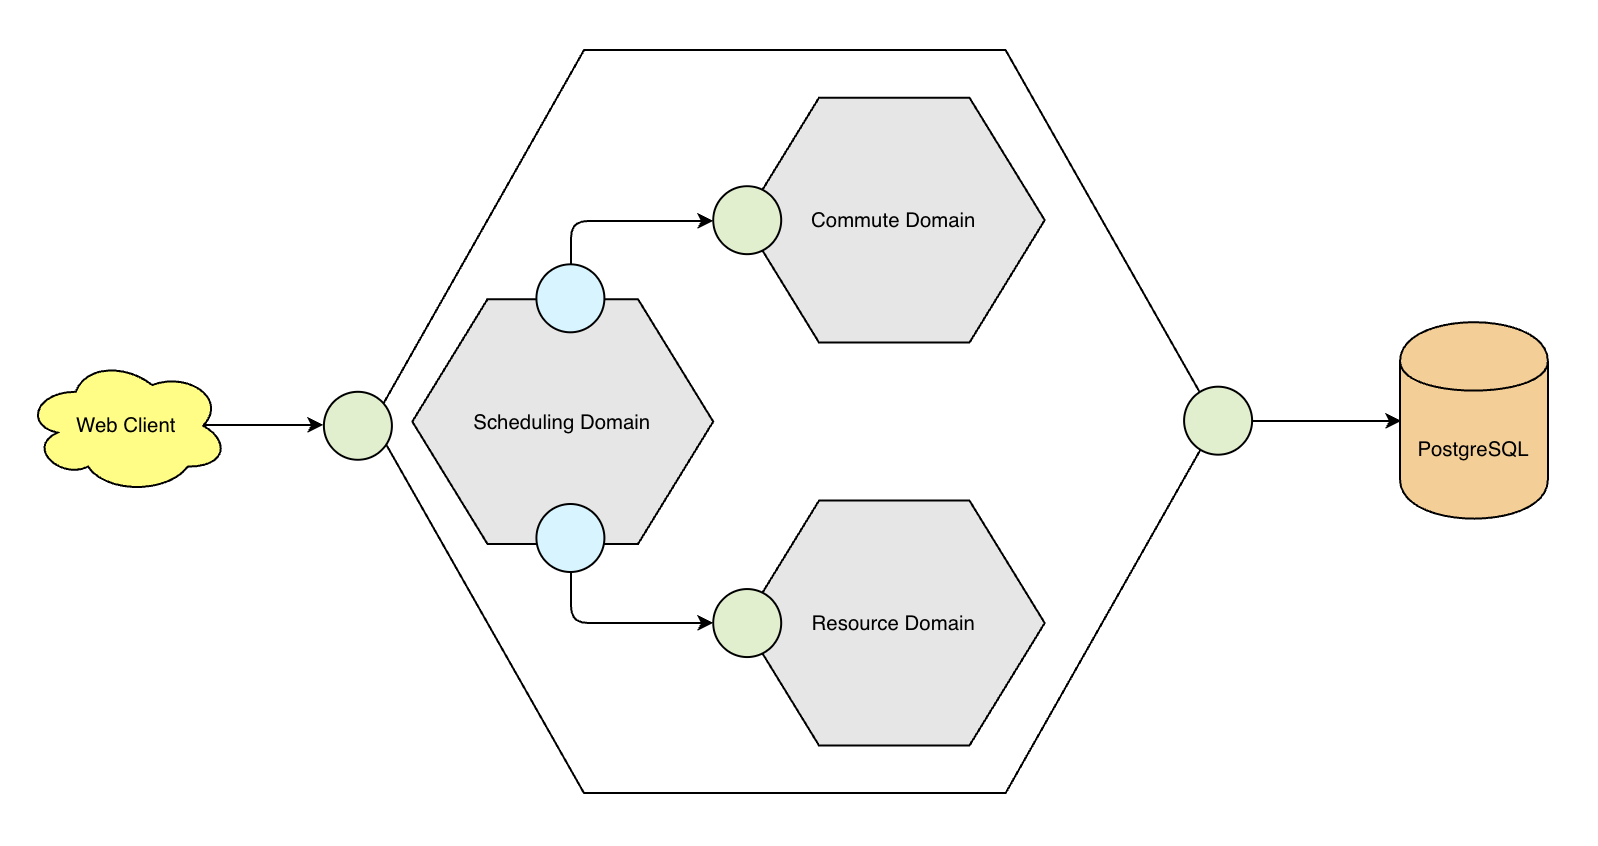
\includegraphics[width=1\textwidth]{images/converge_hexa.png}
\end{center}
\textbf{2.Modular Monolith Deployment Architecture}
\begin{center}
    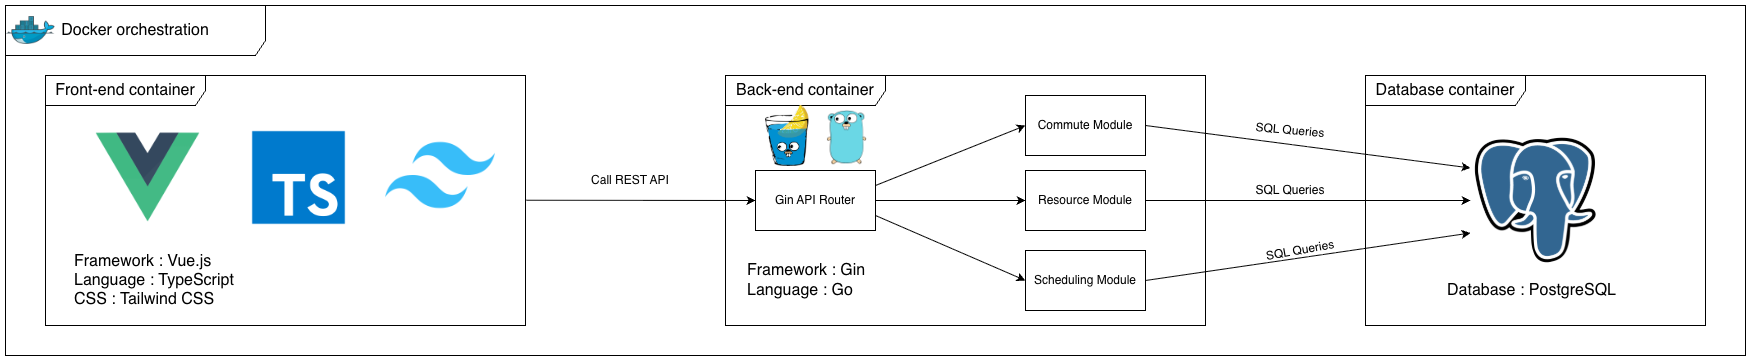
\includegraphics[width=1\textwidth]{images/converge_monolith.png}
\end{center}
\subsection{Use Case Diagram}
\begin{center}
    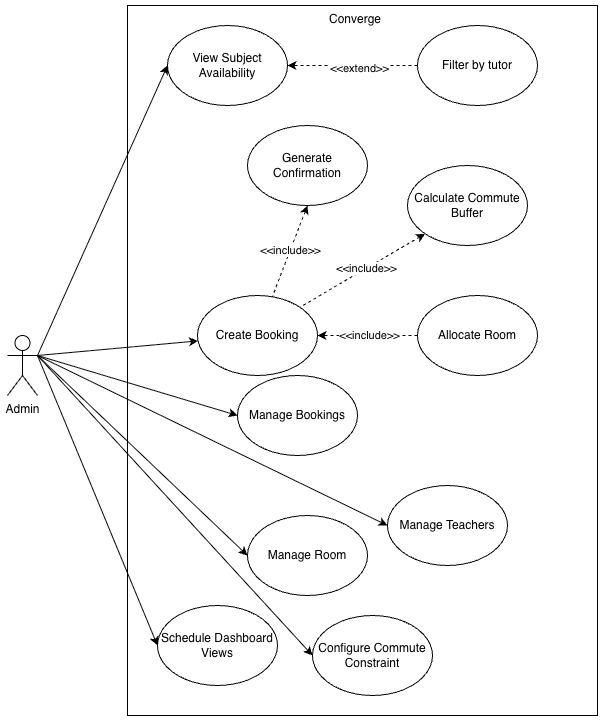
\includegraphics[width=1\textwidth]{images/converge_usecase.png}
\end{center}

\newpage
\subsection{Product Features}
\subsubsection{Smart Booking Engine}
\textbf{Description:} Automatically matches parent/student requests with valid instructors, time slots, and rooms. \\
\textbf{Actor:} Admin \\
\textbf{Details:}
\begin{itemize}
    \item \textbf{Request Input:}
    \begin{itemize}
        \item Admin must input subject and branch to initiate the search.
        \item Selection of a Preferred Time and Specific Instructor is optional, allowing the system to suggest all available possibilities.
    \end{itemize}
    
    \item \textbf{Constraint-Based Filtering:}
    \begin{itemize}
        \item Filters instructors based on availability, and subject expertise.
    \end{itemize}
    
    \item \textbf{Auto Suggestion:}
    \begin{itemize}
        \item Displays only valid booking options in real-time.
        \item Suggests alternative instructors or time if the specific request is unavailable.
    \end{itemize}
    
    \item \textbf{Booking Confirmation:}
    \begin{itemize}
        \item Automatically generates a digital summary of the finalized schedule once a booking is created.
    \end{itemize}
\end{itemize}

\subsubsection{Commute-Aware Scheduling}
\textbf{Description:} Enforces travel time whenever an instructor needs to change branch locations. \\
\textbf{Actor:} Admin \\
\textbf{Details:}
\begin{itemize}
    \item \textbf{Travel Buffer Enforcement:}
    \begin{itemize}
        \item Automatically shifts the next available start time forward by the fixed duration.
    \end{itemize}
    
    \item \textbf{Deterministic Logic:}
    \begin{itemize}
        \item Uses predefined travel times between branches or a default of 30 minutes.
    \end{itemize}
    
    \item \textbf{Visual Buffer Integrity:}
    \begin{itemize}
        \item The master schedule displays the commute as a specific \enquote{Travel Needed} making it clear to the administrator why a tutor's availability has been shifted.
    \end{itemize}
\end{itemize}

\newpage
\subsubsection{Automatic Room Management}
\textbf{Description:} Allocates and manages classroom resources automatically. \\
\textbf{Actor:} Admin \\
\textbf{Details:}
\begin{itemize}
    \item \textbf{Room Management:}
    \begin{itemize}
        \item Provides an interface to add new branch locations and modify rooms of existing branches.
    \end{itemize}

    \item \textbf{Branch Travel Configuration:}
    \begin{itemize}
        \item Provides an interface for administrators to define and modify custom travel times between specific branch pairs. Any pair without a custom value automatically falls back to the system-wide default of 30 minutes.
    \end{itemize}
    
    \item \textbf{Standardized Allocation:}
    \begin{itemize}
        \item Automatically pairs every booking with any available room at the target branch.
    \end{itemize}
    
    \item \textbf{Capacity Feedback:}
    \begin{itemize}
        \item Explicitly displays a \enquote{No Room Available} status for time slots where all physical spaces at a branch are already occupied.
    \end{itemize}
\end{itemize}

\subsubsection{Centralized Schedule Dashboard}
\textbf{Description:} Provides a unified interface to manage all schedules. \\
\textbf{Actor:} Admin \\
\textbf{Details:}
\begin{itemize}
    \item \textbf{Instructor Booking List:}
    \begin{itemize}
        \item Displays a structured list of all teachers and their complete set of booked classes across all dates.
    \end{itemize}
    
    \item \textbf{Alternative Visualizations:}
    \begin{itemize}
        \item Provides a toggleable calendar view as a visual alternative to the text-based assignment list.
        \item Displays commute buffers as explicit non-teaching blocks to ensure logging accuracy.
    \end{itemize}
    
    \item \textbf{Operational Filtering \& Management:}
    \begin{itemize}
        \item Enables filtering by specific instructor or branch.
        \item Includes the administrative interface for managing teachers and booking. 
    \end{itemize}
    
    \item \textbf{Commute Time Configuration:}
    \begin{itemize}
        \item Provides the interface for administrators to manage global system settings, such as modifying default commute constraints. 
    \end{itemize}
\end{itemize}

\newpage
\subsection{SDLC}
Based on our project scope and team size, we decided to use Agile methodologies. It is perfectly suited for a small, remote team like ours that is still in the learning phase and operating under short deadlines. Agile provides the exact flexibility we need to adapt and succeed.

After confirming Agile as our foundation, we chose to implement a Kanban + XP hybrid style. Kanban tells us what to work on next, while XP tells us how to write it well. Neither alone is enough, but together, they cover everything a 2-person remote team needs to deliver high-quality software.

Furthermore, we realized that a Continuous Flow (Kanban) fits our dynamics much better than fixed 2-week sprints. Since our team members have varying schedules and features naturally finish at different speeds, continuous flow allows us to pull work asynchronously without blocking each other's progress.

\subsection{Limits}
\begin{enumerate}
    \item \textbf{Administrative Access Only:} The system is designed as a back-office tool for center managers. It does not include a student-facing portal, tutor login accounts, or self-service booking interfaces for parents.
    \item \textbf{Non-Financial Scope:} The application does not handle any monetary transactions, including tuition fee collection, payroll processing for tutors, or tax invoicing.
    \item \textbf{No Automated External Notifications:} While the system calculates the optimal schedule, it does not send automated Email, or LINE messages. All communication with parents and tutors remains a manual process handled by the admin.
    \item \textbf{Fixed Time Commute Logic:} Commute buffers are calculated based on a configurable branch-pair matrix rather than real-time traffic data, eliminating dependency on external APIs. A default of 30 minutes applies to any pair without a custom value defined.
    \item \textbf{Single Organization Focus:} The architecture is designed for a single tutoring business with multiple physical branches. it is not a multi-tenant SaaS for multiple independent companies.
\end{enumerate}

\newpage
\subsection{Milestones}

\textbf{Phase 1: Proposal} — (30 March 2026 - 10 April 2026)\\
\mytable{|X[1.2,l]|X[l]|X[l]|X[l]|X[l]}{
Task & Start Date & End Date & Duration & Responsibility \\

Project Proposal & 
19 March 2026 &
10 April 2026 &
23 days &
PT, SP
\\

Topic defined &
19 March 2026 &
10 April 2026 &
23 days &
PT, SP
\\

Topic reviews &
21 March 2026 &
23 March 2026 &
3 days &
PT, SP
\\

Proposal submit &
24 March 2026 &
24 March 2026 &
1 days &
PT, SP
\\

Prepare for the presentation &
25 March 2026 &
29 March 2026 &
5 days &
PT, SP
\\

Proposal presentation &
30 March 2026 &
10 April 2026 &
12 days &
PT, SP
\\

Proposal submission &
24 April 2026 &
24 April 2026 &
1 days &
PT, SP
\\
}
\begin{center}
    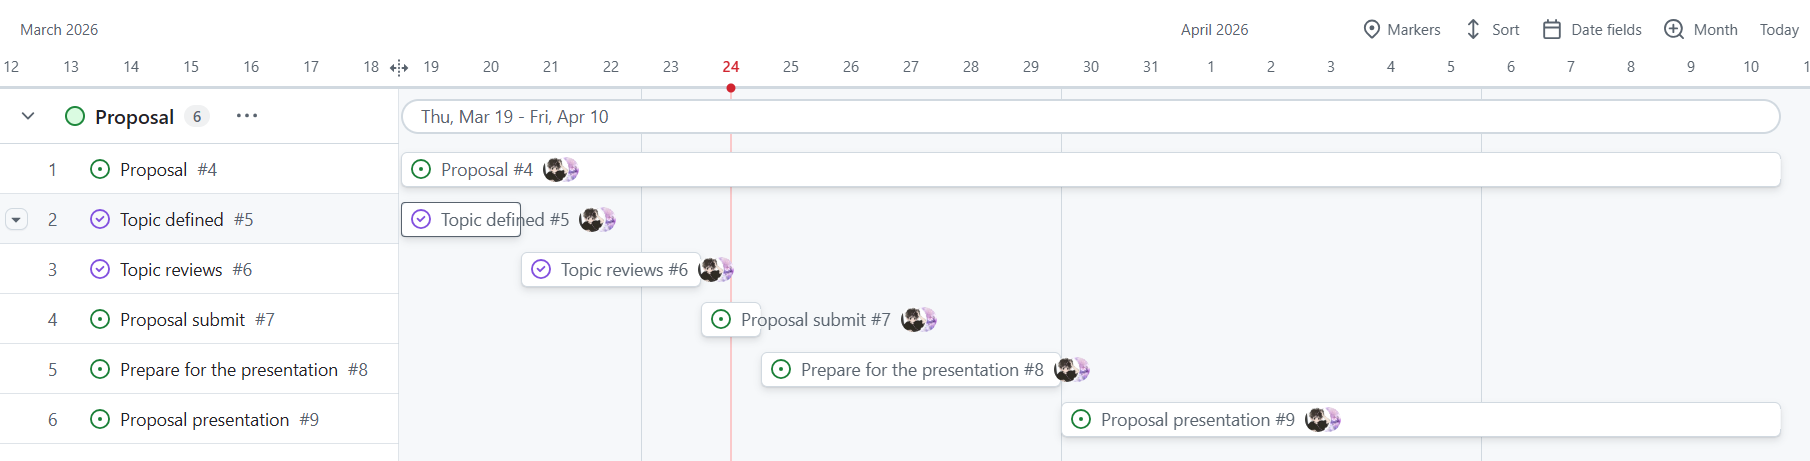
\includegraphics[width=1\textwidth]{images/timeline_proposal.png}
\end{center}

\newpage
\textbf{Phase 2: Progress I} — (15 April 2026 - 21 June 2026 2026)\\
\mytable{|X[1.2,l]|X[l]|X[l]|X[l]|X[l]}{
Task & Start Date & End Date & Duration & Responsibility \\

Setup Project Infrastructure &
15 April 2026 &
25 April 2026 &
11 days &
PT, SP
\\

Core Feature 1: Smart Booking Engine &
26 April 2026 &
25 May 2026 &
14 days &
PT, SP
\\

Core Feature 3: Automatic Room Management &
26 May 2026 &
12 June 2026 &
18 days &
PT, SP
\\

Prepare for Progress I &
13 June 2026 &
17 June 2026 &
5 days &
PT, SP
\\

Progress I Presentation &
18 June 2026 &
21 June 2026 &
4 days &
PT, SP
\\

}
\begin{center}
    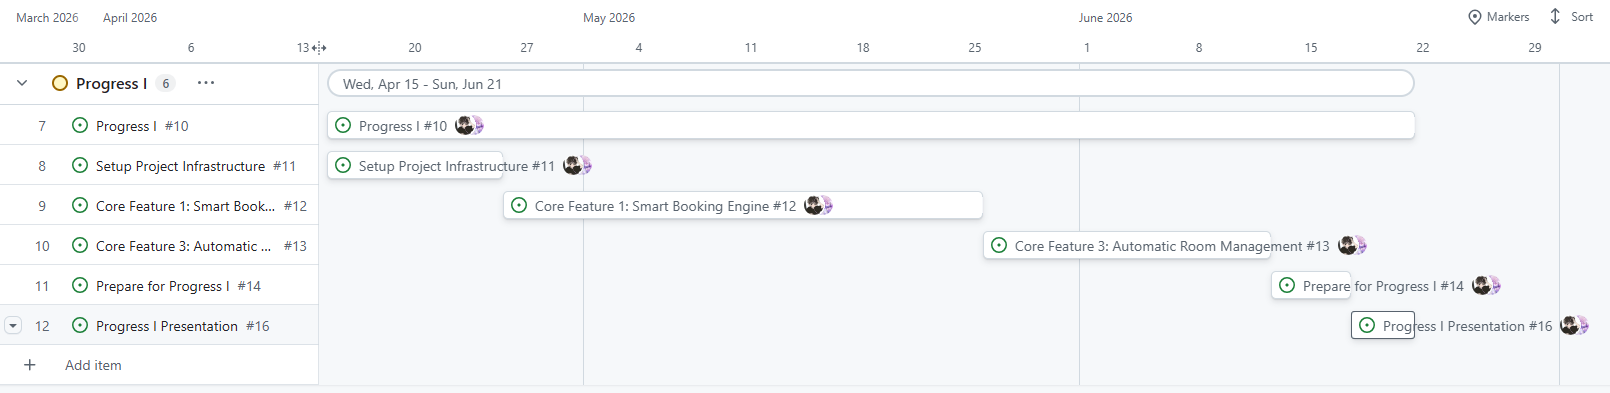
\includegraphics[width=1\textwidth]{images/progress1.png}
\end{center}

\newpage
\textbf{Phase 3: Progress II} — (22 June 2026 - 30 September 2026) \\
\mytable{|X[1.2,l]|X[l]|X[l]|X[l]|X[l]}{
Task & Start Date & End Date & Duration & Responsibility \\

Core Feature 3: Travel Buffer System &
1 July 2026 &
10 July 2026 &
10 days &
PT, SP
\\

Core Feature 4: Branch Capacity Monitoring &
11 July 2026 &
20 July 2026 &
10 days &
PT, SP
\\

Core Feature 5: Interactive XAI Decision Dashboard &
21 July 2026 &
30 July 2026 &
10 days &
PT, SP
\\

Core Feature 6: Automated Disaster Recovery &
31 July 2026 &
9 August 2026 &
10 days &
PT, SP
\\

Prepare for Progress II &
10 August 2026 &
16 August 2026 &
7 days &
PT, SP
\\

Progress II Presentation &
17 August 2026 &
21 August 2026 &
5 days &
PT, SP
\\
}
\begin{center}
    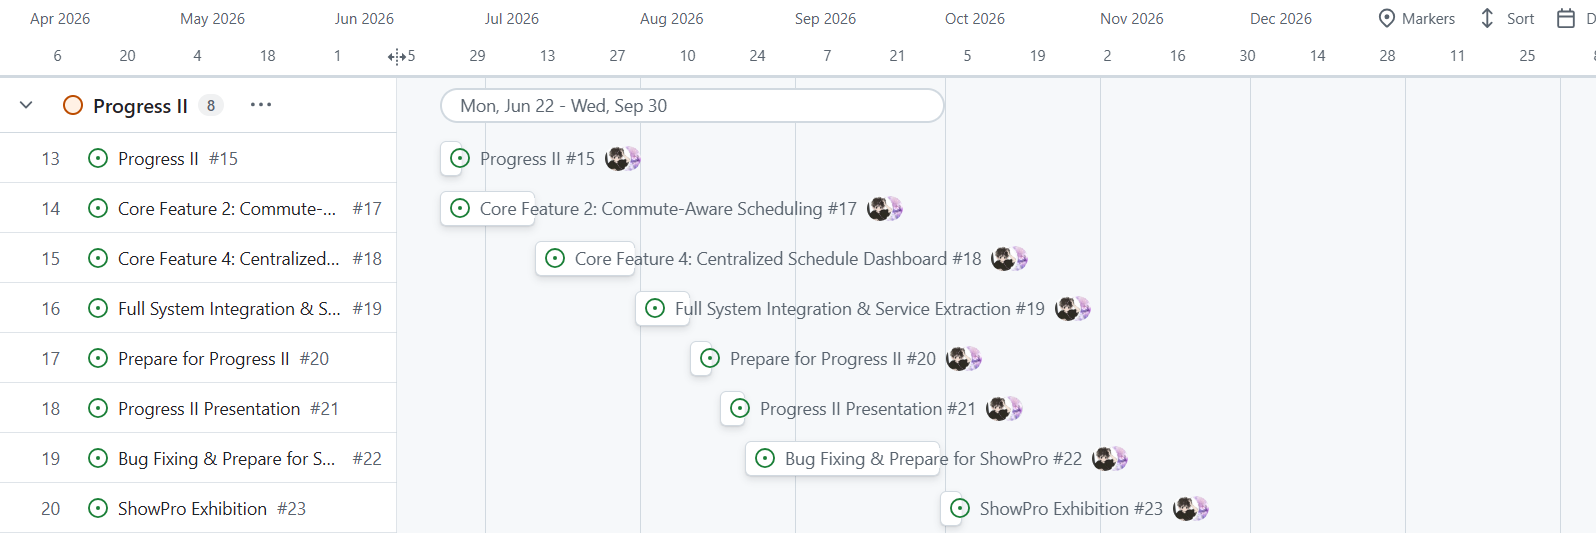
\includegraphics[width=1\textwidth]{images/progress2.png}
\end{center}

\newpage
\textbf{Phase 4: Final Progress} — (1 October 2026 - 2 November 2026)\\
\mytable{|X[1.2,l]|X[l]|X[l]|X[l]|X[l]}{
Task & Start Date & End Date & Duration & Responsibility \\

Quality Assurance &
1 October 2026 &
7 October 2026 &
7 days &
PT, SP
\\

System Documentation &
8 October 2026 &
14 October 2026 &
7 days &
PT, SP
\\

Prepare Final Presentation &
15 October 2026 &
18 October 2026 &
4 days &
PT, SP
\\

Final Progress Presentation &
19 October 2026 &
2 November 2026 &
15 days &
PT, SP
\\
}
\begin{center}
    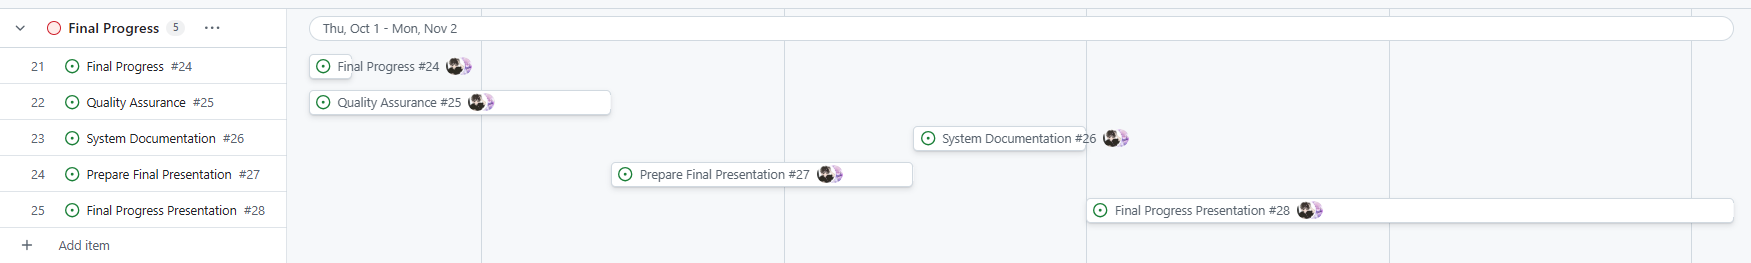
\includegraphics[width=1\textwidth]{images/final_progress.png}
\end{center}

\newcommand{\cmark}{\ding{51}}

\renewcommand{\arraystretch}{1.3}

\begin{tabularx}{\textwidth}{|X|c|c|}
\hline

\multirow{2}{*} 
& \multicolumn{2}{c|}{\textbf{Pct of task complete (\%)}} \\
\cline{2-3}
& \textbf{Progress I} & \textbf{Progress II} \\
\hline

\textbf{Feature 1: Automated Data Ingestion Form} & 0\% & 0\% \\
\hline

1.1 Structured Input &  & \\
1.2 Data Normalization&  & \\
\hline

\textbf{Feature 2: Constraint Satisfaction AI Engine} & 0\% & 0\% \\
\hline

2.1 Request Input &  & \\
2.2 Constraint-Based Filtering &  & \\
2.3 Heuristic Auto-Suggestion &  & \\
2.4 Explainable AI (XAI) Trace Logs &  & \\
\hline

\textbf{Feature 3: Travel Buffer System} & 0\% &  0\%\\
\hline

3.1 Buffer Configuration &  & \\
3.2 Deterministic Injection &  & \\
3.3 Visual Buffer Integrity &  & \\
\hline

\textbf{Feature 4: Branch Capacity Monitoring} & 0\% &  0\%\\
\hline

4.1 Capacity Definition &  & \\
4.2 Concurrent Tracking &  & \\
4.3 Capacity Feedback \& Prevention &  & \\
\hline

\textbf{Feature 5: Interactive XAI Decision Dashboard} & 0\% &  0\%\\
\hline

5.1 Master Schedule View &  & \\
5.2 Operational Filtering &  & \\
\hline

\textbf{Feature 6: Automated Disaster Recovery} & 0\% &  0\%\\
\hline

6.1 Asynchronous Snapshots &  & \\
6.2 Rapid Restoration &  & \\
\hline

\end{tabularx}